\section{Ausgangszustand}
Zum Beginn dieser Arbeit wurde bereits in meiner vorangegangen Tätigkeit bei der Hoffmann Group auf Basis des NRF52840-Dongle prototypisch eine Anwendung implementiert, die auf das Bluetooth Modul der Hoffmann Group aufbaut und zusammen mit diesem die Basis für die Anwendung des Fußschalters darstellt. Dieser Proof-of-Concept Prototyp sollte vorallem zeigen, dass es möglich ist eine Anwendung auf dem selben Chip wie das Bluetooth Modul und das Softdevice laufen zu lassen, die in der Lage ist einerseits ein Massenspeichermedium und einen virtuellen COM-Port öffnet und andererseits über \ac{BLE} mehrere \ac{HCT}Werkzeuge verbindet. Als solche war sie ein voller Erfolg und schaffte die Bereitschaft des Projektmanagements die Ressourcen für die Implementierung des Fußschalters zu bewilligen.\\
In diesem Kapitel wird die Funktionalität und der Aufbau der Dongle-App, sowie die notwendigen Änderungen und Verbesserungen die durchgeführt werden sollen, vorgestellt. Damit soll auch die Implementierungen für den Fußschalter von den bestehenden abgegrenzt werden.

\subsection{Dongle-App}
Die Anwendung nutzt das Bluetooth Modul der Hoffmann Group. Es stellt dabei die Anwendungsschicht des \ac{BLE}-Stack da und abstrahiert somit die \ac{BLE} spezifischen Aufrufe zum Softdevice. Es wird in allen \ac{HCT}-Werkzeugen eingesetzt, wo es eine Vermittlerfunktion zwischen dem eigentlichen Gerätechip und dem Softdevice übernimmt, dabei kann es sowohl in peripheral und central Rolle agieren. Es führt den Verbindungsprozess zu Computern und \ac{HCT}-Geräten durch. Als Softdevice wird das S140 von Nordic Semiconductor in der Version 7.2.0 verwendet. \\
Auf diesem Basisprojekt aufbauend befindet sich die \ac{USB}-Dongle App. Im Gegensatz zu den \ac{HCT}-Werkzeugen sitzt die gesamte Anwendung ebenfalls auf dem Chip des Softdevice und muss sich die Chipressourcen mit ihm teilen. Die Funktionalität, die in dem File usb\_dongle\_app.c gekapselt ist, ist dafür zuständig das Konfigurationsfile einzulesen und die zugehörigen Daten während der Laufzeit zu halten. Dabei handelt sich es um die zu verbindenden \ac{HCT}-Gerät, welche in einer gleichnamigen Struktur mit Name, Seriennummer und einer Kanalzuweisung gespeichert werden. Die Kanalzuweisung wird für das MUX50 bzw. DMX16 Protokoll benötigt. Die Protokolle MUX50 bzw. DMX16 sind dabei proprietäre, \ac{ASCII}-basierte Protokolle und stellte jeweils nur eine leichte Variation des Anderen da. Sie werden benötigt um die Daten an \ac{CAQ}-Software weiterzugeben, welche die Messdaten speichern und auf ihre Richtigkeit überprüfen kann. Werden die Geräte dann verbunden, muss weiterhin der Verbindungszustand, sowie das Connection-Handle gespeichert werden. Des weiteren sammelt es die Messdaten auf, die vom Central Device von den \ac{HCT}-Geräten im Interrupt-Kontext empfangen werden und reiht die Daten, die von Interesse sind, in eine \ac{FIFO} Nachrichtenqueue ein. Diese werden später aus dem Kontext der Main-Loop heraus, in das MUX50 bzw. DMX16 Protokoll umgewandelt und über den virtuellen COM-Port verschickt. Ebenfalls in der Funktionalität des usb\_dongle\_app.c Files und aus dem Kontext des Main-Loop heraus, werden die Befehle des MUX50 Protokolls, welche über dem virtuellen COM-Port empfangen wurden, verarbeitet.\\
In dem File usbd\_msc\_cdc\_composite.c werden \ac{USB} spezifischen Aufrufe gekapselt. Hier wird das \ac{MSC} und der virtuelle COM-Port (\ac{CDC}) initialisiert und konfiguriert. Der Code wurde nur mit kleinen Änderungen aus den Beispielen des NRF\_SDKs übernommen, weswegen nicht weiter auf die Implementierung eingegangen wird.\\
Da es keine Unterstützung seitens der NRF Bibliothek für den internen Flash als Speichermedium für das \ac{MSC} gibt, musste der Treiber block\_device\_ram.c angepasst werden. Er wurde als block\_dev\_fStorage.c in das Projekt gezogen und ruft die Funktionen des Files fStorage.c auf, welches die Schreibbefehle im Interrupt-Kontext ebenfalls in eine \ac{FIFO} Nachrichtenqueue einreiht. Das ist nötig, da für die korrekte Ausführung auf Interrupts des Flash Memory gewartet werden muss, welche nur im Kontext der Main-Loop korrekt empfangen werden. Zudem wird dort Flash Memory spezifische Logik abstrahiert. So muss eine Flash Page erst "erased" werden, bevor sie geschrieben werden kann und die Block Logik des \ac{MSC} wird auf die Flash Page Logik des Speichers übertragen.

\begin{figure}[H] 
	\centering
	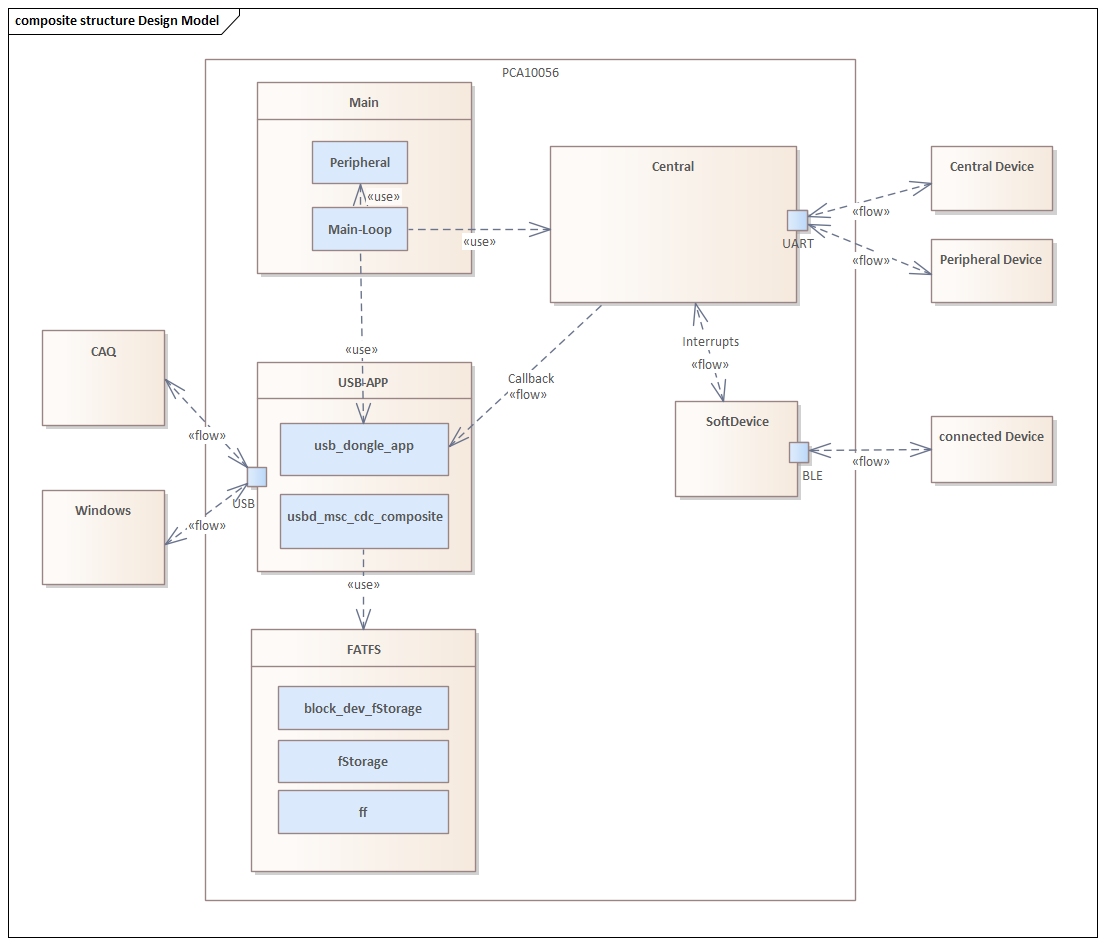
\includegraphics[width=\textwidth]{figures/Design_Model.png}
	\caption{Aufbau des Projekts im Ausgangszustand}
\end{figure}


\subsection{Erweiterungen für Fußschalter}
Für den Fußschalter muss die bestehende Software wie folgt erweitert werden. Die Peripherie des Fußschalter muss eingebunden werden. Diese umfasst den Schalter der durch den Anwender betätigt werden kann, eine LED-Leuchte und den Akku des Fußschalters. In Hinblick auf den Akku muss eine Energiemanagement geschaffen werden, um dessen Kapazität zu schonen. Während die Dongle-App die Daten ausschließlich über den virtuellen COM-Port zur Verfügung stellt, soll im Fußschalter die Art der Ausgabe konfigurierbar sein. Des Weiteren müssen die Schreibbefehle des \ac{MSC} optimiert werden, da sie nur sehr langsam und fehlerbehaftet abgearbeitet werden. Die Änderungen an der Konfiguration der Anwendung wird außerdem erst übernommen, wenn der Dongle abgezogen und wieder angesteckt wird, also die Anwendung neugestartet wird. Beim Fußschalter sollen Änderungen an den Konfigurationsfiles detektiert werden und die Anwendung programmatisch neugestartet werden, auch weil durch den Akku die Anwendung durch den Nutzer nicht direkt neugestartet werden kann. Es müssen außerdem die Messuhren bzw. Messschieber eingebunden werden. Zusätzlich soll die Anwendung weiterhin auch als Dongle erhältlich gemacht werden und die Implementierung muss in Hinblick auf diese Hardwarunterschiede durchgeführt werden.

\subsection{Überarbeitung der Dongle-App}
Der Prototyp der Dongle-App zeigte, dass die genannten Funktionalitäten technisch möglich sind. Für den Fußschalter sollen sie evaluiert und wenn nötig verbessert werden. Zudem sollen die verschiedenen Projekte, die sich durch die Implementierung des Fußschalters ergeben, getrennt werden.

\subsubsection{Trennung der Projekte}
Durch die Entwicklung des Fußschalter entstehen drei verschiedene Projekte, deren Code sich jeweils stark überschneidet. Dabei müssen Updates und Änderungen für eines der Projekte mit einem möglichst geringen Aufwand auch in die anderen übernommen werden. Insbesonders die Updates für das Framework der Hoffmann Group zur Abstraktion der \ac{BLE}-Schnittstelle nrf\_Base müssen, um die fehlerfreie Kommunikation des Fußschalters zu den \ac{HCT}-Werkzeugen sicherzustellen, in die Projekte des Dongles und des Fußschalters übernommen werden. Es wird in allen \ac{HCT}-fähigen Produkten eingesetzt und stetig weiterentwickelt und darf unter keinen Umständen den Code der anderen Projekte nicht beeinhalten. Auch muss berücksichtigt werden, dass die Projekte jeweils unterschiedliche Peripherie benötigen.\\
Folgende Peripherie darf dabei nur in den jeweiligen Projekten initialisiert werden:
\begin{itemize}
	\item nrf\_Base: \ac{UART}
	\item Dongle: Ein-Farben LED, \ac{USB}
	\item \ac{HCT}-FootSwitch: Fußtaster, Akku Power Management, Drei-Farben LED, \ac{USB}
\end{itemize}

Um diese Anforderungen zu erfüllen kann einerseits für alle drei Projekte eine eigene Codebasis geschaffen werden, die sich jeweils stark überschneiden und gesondert gepflegt werden müssen oder die selbe Codebasis für alle Projekte benutzt werden. Die erste Möglichkeit hat den Vorteil, dass sich die Entwicklung einfacher gestaltet, da auf diese Abhängigkeiten keine Rücksicht genommen werden muss. Zudem kann der Code stärker auf den Anwendungsfall optimiert werden, jedoch macht der enorme Arbeitsaufwand die gesonderten Codebasen zu unterhalten und auf dem neuesten Stand zu halten, diese Möglichkeit unpraktikabel. Des weiteren wurde aus Software architektonischen Gründen die Anwendung bereits gekapselt, wodurch die programmatische Abtrennung der Teile keinen außerordentlichen Entwicklungsaufwand erfordert.\\
Stattdessen muss aus der Main-Routine nur zwei Funktionsaufrufe mit Compilerschaltern abgetrennt werden, um den Code des Fußschalter bzw. Dongles vom nrf\_Base Projekt zu trennen. Zum einen der Initialisierungsaufruf und ein App-process Aufruf, da der Main-Loop als Dispatcher für die gesamte Anwendung fungiert. Im Central müssen die Datencallbacks, sowie im Connection State Callback die Aufrufe an die Dongle-App abgetrennt werden. Die Funktionalität der \ac{UART} stellte sich als wenig gekapselt heraus und musste an zahlreiche Stellen kleinteilig aus dem Fußschalterprojekt abgetrennt werden.\\ 
Das ambitioniertes Ziel war dabei, dass nach der Einführung der Compilerschalter das Binärfile des nrf\_Base Projekts identisch zu der vorangegangenen Version ohne Fußschalter sein sollte. Aus noch nicht geklärten Umständen ist das jedoch nicht der Fall.


\subsubsection{Verbesserung Verbindungsaufbau}
Im Ausgangszustand der Dongle-App werden lediglich zwei Zustände im Verbindungsaufbau abgebildet: ``unconnected'' und ``connected''. Aus der Zuordnung des Connection Handles, also dem Wechsel dieser Variable aus dem Default Wert 0xFFFF auf einen beliebigen anderen Wert, kann zusätzlich darauf geschlossen werden, dass die Service Discovery abgeschlossen wurde und mit der Subscription begonnen werden kann. Diese Abbildung des Verbindungsaufbaus ist mehrer Hinsicht unvollständig.\\
Der Zustand ``connected'' in der Dongle-App bildet den Zustand fehlerhaft ab. Er wird eingenommen, sobald ein erster Verbindungsaufbau durch die Anwendung angestoßen wurde. Zum diesen Zeitpunkt ist noch keine Kommunikation über die Scan Response hinaus erfolgt und folglich kann noch kein Connection Handle dem zu verbindenden Gerät zugeordnet werden. Im nrf\_Base Framework wird dieser Zustand, getriggert durch das korrespondieren Event, erst nach der initialen Kommunikation eingenommen und das Connection Handle ist bereits zugeordnet. Das ist ein entscheidender Unterschied, da ab diesem Zeitpunkt ein Verbindungsabbruch auftreten und nur über das Connection Handle nachvollzogen werden kann. Das kann dazu führen, dass im Werkzeug der Verbindungsaufbau fehlgeschlagen ist, jedoch in der Dongle-App das Gerät im Zustand ``connected'' ohne Connection Handle festhängt. Nicht nur wird dieses Wekrzeug nicht mehr vollständig verbunden, sondern solange es in diesem Zustand bleibt, wird bei keinem anderem Gerät ein Verbindungsaufbau angestoßen.\\
Wenn die Service Discovery ausgeführt wurde, wird in der Dongle-App mit diesem Event das Connection Handle zugeordnet und die Subscription angestoßen. Mit dieser Zuordnung ist in der Dongle-App das Gerät vollständig verbunden und die derzeitig eingestellte Messeinheit des Werkzeugs wird abgefragt. Dabei wird jedoch nicht darauf gewartet, dass das zu einer erfolgreichen Subscription korrespondieren Acknowledgement erhalten und der Zustand ``Subscription'' eingenommen wurde. Auch hier können bei einer fehlgeschlagenen Subscription Fehler in der Anwendung auftreten.\\
Die Zustände des Verbindungsaufbaus sollen jetzt korrekt und vollständig in der Anwendung abgebildet werden. Dabei wurde die Callback Funktionen bisher direkt im Eventhandler des Central aufgerufen. Diese Erweiterung hätte es erfordert, eine respektiven Callback in allen zugehörigen Events aufzurufen, was entgegen der Kapselung der Projekte geht. Jedoch gibt es im Central bereits eine ähnliche Funktionalität, die den Zustand des Central Moduls über \ac{UART} ausgibt und bereits in den Events des Verbindungsaufbaus aufgerufen wird. Sie wird nun erweitert, sodass falls der Compilerschalter für die \ac{USB}-App gesetzt ist, der Zustand des Moduls nicht über \ac{UART}, sondern an einen Callback der \ac{USB}-App überreicht wird. In der \ac{USB}-App wird der Zustand gespeichert und die dazugehörigen Folgeaktionen durchgeführt. Im Central Modul ist weiterhin nur ein einziger Aufruf einer \ac{USB}-App Funktion vonnöten, um die Zustände des Verbindungsaufbaus in der \ac{USB}-App abzubilden.

\begin{figure}[H] 
	\centering
	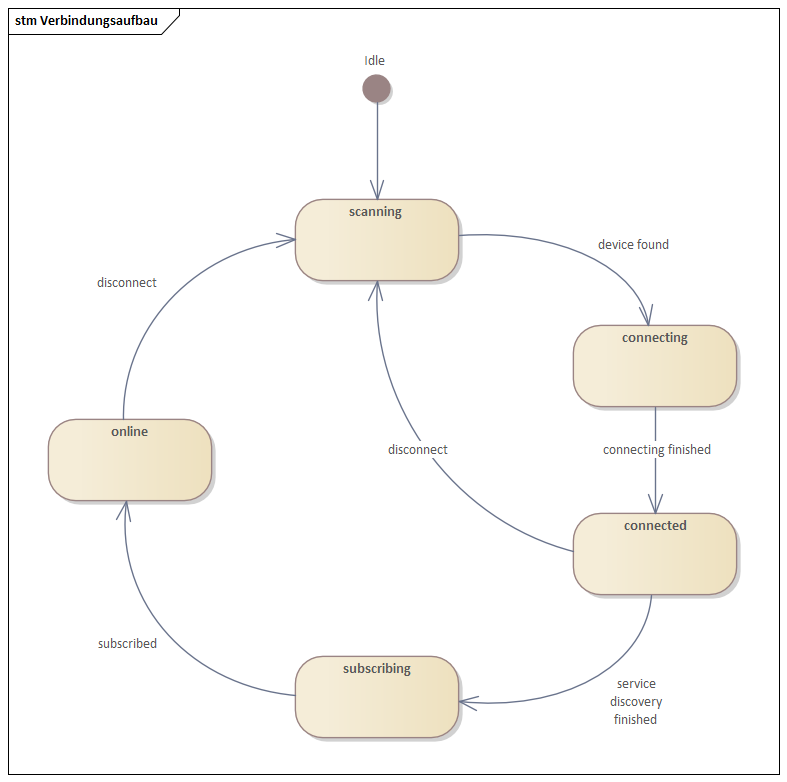
\includegraphics[width=\textwidth]{figures/Verbindungsaufbau.png}
	\caption{Zustandsdiagramm des Verbindungsaufbaus}
\end{figure}



\subsubsection{Optimierung Abfrage Messeinheit}
Jede Nachricht die über \ac{BLE} gesendet wird braucht Rechenleistung und Energie und steigt mit der Anzahl der verbundenen Geräte linear an. Im Ausgangszustand der \ac{USB}-Dongle App muss die Anwendung bei Werkzeug der Marke Holex jedes Mal, wenn sie ein Messergebnis erhält, die Einheit der Messung abfragen. Bei Drehmomentschlüsseln der Marke Garant wird ein Datenblock mit der Messeinheit kurz nach Erhalten des Messergebnisses empfangen. Diese Nachricht bezieht sich jedoch auf die derzeitig eingestellte Messeinheit, welche im Fall eines Arbeitsablaufs mit sich ändernden Einheiten, die Einheit für die nächste Messung ist. In diesem Fall gibt die \ac{USB}-Dongle App die falsche Einheit aus. Bei Geräten der Marke Holex wird nur bei einer Änderung der Messkonfiguration, diese übermittelt.\\
In beiden Fällen sendet das Werkzeug automatisch bei einer Änderung der Messkonfiguration einen Datenblock mit der Messeinheit an die Subscriber der \ac{HCT}-Charakteristik. Die Kontrolle der Messeinheit kann daher verbessert werden, indem die derzeitig eingestellte Messeinheit nach dem Verbindungsaufbau einmal abgefragt wird und für jedes verbundene Gerät gespeichert wird. Bei einer Änderung der Messeinheit erhält die Dongle-App die neue Messkonfiguration und aktualisiert die gespeicherte Einheit. Dadurch wird eine fehlerhafte Einheit in der Ausgabe vermieden, wird damit die Anzahl an Nachrichten der Dongle-App an das Messgerät verringert und die kritischen Ressourcen Rechenleistung und Energie geschont.

\begin{figure}[H] 
	\centering
	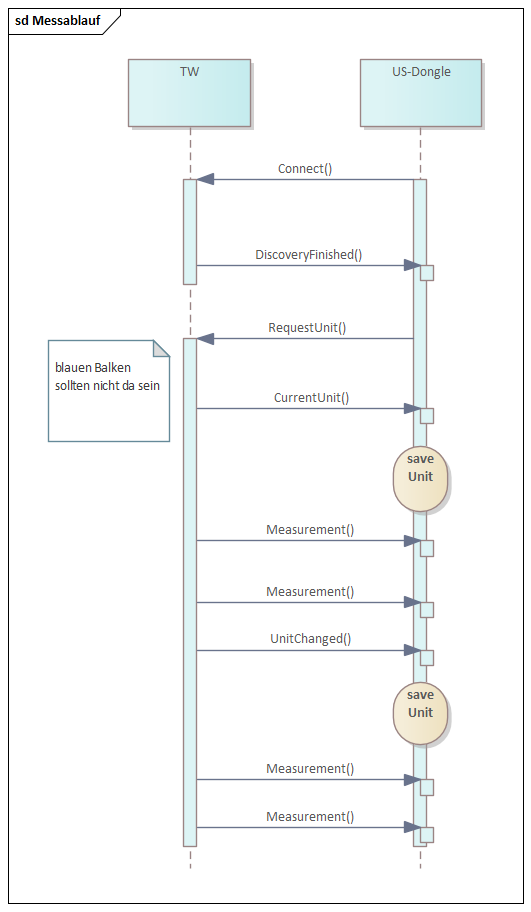
\includegraphics[width=\textwidth]{figures/Messablauf.png}
	\caption{Messablauf}
\end{figure}